\documentclass{beamer}
\usepackage{fontspec,xunicode,xltxtra,beamerthemesplit}
\usepackage{graphicx}
\usepackage{beamerthemeshadow}
%\usepackage{algorithmic}
%\usepackage{algorithm}
\usepackage[CJKmath = true]{xeCJK}
\usepackage{fancyhdr}

\usetheme{Antibes}
%\setsansfont[Mapping=tex-text]{SimSun}
%\setmainfont[BoldFont=Microsoft YaHei]{SimSun}
%\setmonofont{Microsoft YaHei}
\setCJKmainfont[BoldFont=Microsoft YaHei]{SimSun}
%\setCJKmainfont{SimSun}
%\setCJKmathfont{楷体}
%\setCJKsansfont{Times New Roman}


\title{A Deep Architecture for Matching Short Texts}
\author{赵惜墨}
\date{\today}
\institute{哈尔滨工业大学\\计算机学院\\智能技术与自然语言处理实验室}

\XeTeXlinebreaklocale "zh" % 表示用中文的断行
\XeTeXlinebreakskip = 0pt plus 1pt % 多一点调整的空间

\begin{document}



\frame{\titlepage}

\section{bilinear}

\frametitle{bilinear}
从bilinear的模型匹配开始:

\begin{displaymath}
    match(x,y) = x^{T}Ay = \sum_{m=1}^{D_x} \sum_{n=1}^{D_y} A_{nm}x_my_n
\end{displaymath}
  \begin{enumerate}
  \item A是提前计算好的,相当与权重
  \item 每一个子元素的乘积$x_ny_m$都可以看作是一个$x和y的$局部决策(local decision)。
  \item 上面加和的向量积$M=xy^{T}$可以看作是$x和y$的部分决策的空间表示。最终的决策考虑了所有的局部决策,因此在bilinear 中有:$\emph{match} = \sum_{nm}A_{nm}M_{nm}$,也就是所有局部权重的线性加和。
  \end{enumerate}
  
}

\section{from linear to deep}

\frame{
\frametitle{概念}
\begin{description}
\item[parallel text] 需要匹配的两个文本(问答)对
\item[局部性] 在底层用词的共现(co-occurrence)来匹配语义。
\item[混合性] 决策有不同层次的抽象。局部决策,抓住词义相近的词之间的关
系,将会逐层形成最后和全局决策。
\end{description}

}

\frame{
  \frametitle{localness}

  局部匹配与图像匹配相类似,平行文本的文本块由两个文本之间的关联词决定。像处理图像一样,可以用$(\Omega_{x,p},\Omega_{y,p})$来决定匹配的范围,$(\Omega_{x,p},\Omega_{y,p})$分别代表$X,Y$的子集。与图像一样,用块“patch”来表示。

  \begin{figure}
  \centering
  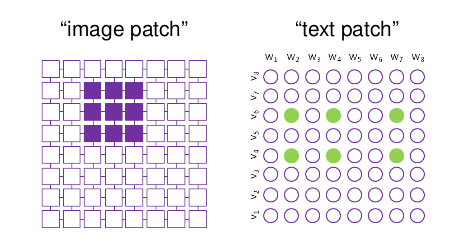
\includegraphics[height=3cm,width=5cm]{imagetext.png}
  \caption{fig:图像块vs文本块}
  \label{fig:patch}
\end{figure}

}

\frame{
  \frametitle{localness 续}

  \begin{enumerate}
  \item 文本块不能用给定的连续空间。因为词不一定和其周围词相关,因此需要通过匹配文本的共现对来发现。
  \item 用bilingual topic model来发现共现对,这种方法可以成功获取同领域和不同领域的共现对,这种方法可以成功获取同领域和不同领域的共现对。基本的思想是:
    \begin{enumerate}
    \item 当词对多次在跨领域出现的时候(例如,感冒——抗体),它们在决定匹配的时候有很高的得分
    \item 当词对多次在相同领域出现的时候(例如,夏威夷——度假),它们对该领域匹配有很高的帮助。
    \item 例如,从QA对中就可以发现,夏威夷和RAM就不可能作为一个共现对。也就是说,模型只在块中匹配底层次的语义关系。
    \end{enumerate}
  \end{enumerate}
}

\frame{
  \frametitle{形成层次性的决策过程}
  \begin{columns}
    \begin{column}{0.3\textwidth}
      \begin{figure}
        \centering
        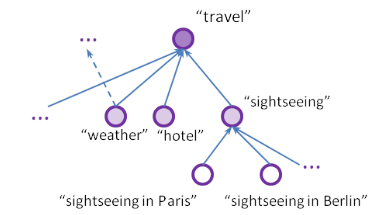
\includegraphics[height=3cm,width=4cm]{gao.png}
          \caption{层次决策}  
        \label{fig:viterbi}
      \end{figure}
    \end{column}
    \begin{column}{0.7\textwidth}
      \begin{enumerate}
      \item 决策完成之后,大多数词之间的相关性都是没有的。
      \item “sightseeing in paris”和“sightseeing in berlin”
      \item “sightseeing”来形成一个更高的决策。
      \item 也能够相对的形成“hotel”和“transportation”,这些都能形成一个更高的层次“travel”。
      \item 注意到高层次主题对底层次主题没有包含关系。
      \end{enumerate}
    \end{column}
  \end{columns}
}

\section{deep architecture}

\frame{
  \frametitle{Topic Modeling for Parallel Texts}
  \begin{enumerate}
  \item 具体方法是用的LDA+Gibbs sampling
  \item 将问答对放到同一篇文章中,对每一个topic建一个词表,避免混合。
  \item 允许词表之间有重叠,例如,希望词(hotel,price)能够出现在不同的topic中。
  \item 按照topic数量,找到逐层递减的topic集合,$H=\{T_1,\cdots ,T_L\}$
  \end{enumerate}
}

\frame{
  \frametitle{如何利用topic}
   \begin{columns}
    \begin{column}{0.3\textwidth}
      \begin{figure}
        \centering
        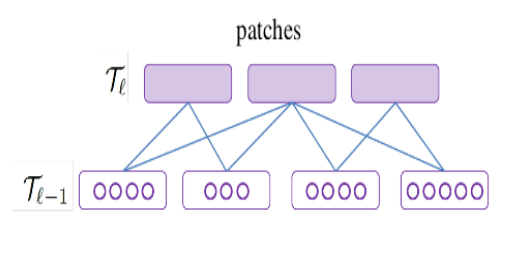
\includegraphics[height=3cm,width=4cm]{topic.png}
          \caption{层次决策}  
        \label{fig:viterbi}
      \end{figure}
    \end{column}
    \begin{column}{0.7\textwidth}
      \begin{enumerate}
      \item 剪掉在所有主题概率都很低的词。剩下的词在每一个主题确定一个块。
      \item 根据H,建立一个DAG G,根据在$T_l$ 和$T_{l-1}$ 共同出现的词,确定连接。
      \item 重复此过程,建立神经网络。
      \end{enumerate}
    \end{column}
  \end{columns}

}

\frame{
  \frametitle{最终得到的模型}

  \begin{figure}
  \centering
  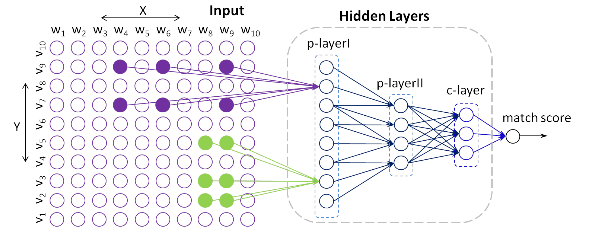
\includegraphics[height=5cm,width=10cm]{jiegou.png}
  \caption{网络结构}
  \label{fig:jiegou}
\end{figure}

}

\frame{
\frametitle{训练}
训练用的BP
}

\frame{
\frametitle{实验}
\begin{figure}
  \centering
  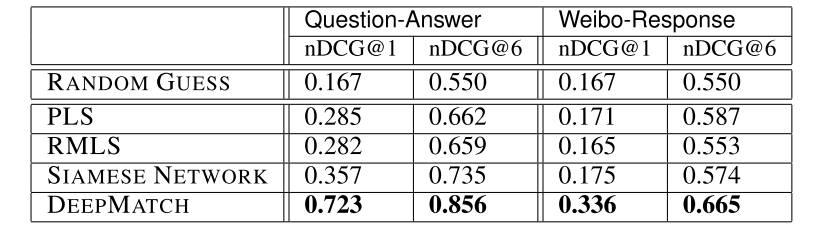
\includegraphics[height=3.5cm,width=10cm]{shiyan.png}
  \caption{实验结果}
  \label{fig:jiegou}
\end{figure}
}

\end{document}
